\documentclass{../LatexStyle/style}

\title{\Large \bf Final Project}

\begin{document}

\maketitle

\begin{instructions}
\textbf{Objective:} \\
Implement a C++ class to represent a perceptron, a fundamental building block of neural networks. You are \textbf{not} required to implement a training algorithm.

\begin{enumerate}
    \item \textbf{Perceptron Class:}
    \begin{itemize}
        \item Implement a class that models a single perceptron.
        \item The perceptron should support at least two classical activation functions (e.g., step, sigmoid, ReLU, tanh). More activation functions are encouraged.
        \item The perceptron should accept a vector of inputs and corresponding weights, plus a bias term.
        \item The class should have methods to compute the output given inputs and weights, and to set or get the weights and bias.
        \item Include a constructor to initialize the perceptron with weights and bias.
    \end{itemize}

    \item \textbf{What is a Perceptron?} \\
    A perceptron is a simple computational unit that takes several inputs, applies weights to them, sums the result, adds a bias, and passes the sum through an activation function to produce an output. It is the basic unit of a neural network.

    \begin{center}
        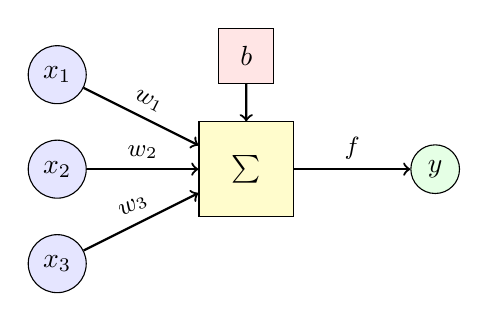
\begin{tikzpicture}[scale=1.2]
            % Inputs
            \foreach \i in {1,2,3} \node[circle,draw,fill=blue!10] (X\i) at (0,2-\i) {$x_{\i}$};
            % Weights
            \node[rectangle,draw,fill=yellow!20,minimum width=1.2cm,minimum height=1.2cm] (P) at (2,0) {\textbf{\huge$\sum$}};
            % Output
            \node[circle,draw,fill=green!10] (Y) at (4,0) {$y$};
            % Connections
            \foreach \i in {1,2,3} \draw[->,thick] (X\i) -- node[above,sloped, font=\small] {$w_{\i}$} (P);
            \draw[->,thick] (P) -- node[above, font=\small] {$f$} (Y);
            % Bias
            \node[rectangle,draw,fill=red!10,minimum width=0.7cm,minimum height=0.7cm] (B) at (2,1.2) {$b$};
            \draw[->,thick] (B) -- (P);
        \end{tikzpicture}
    \end{center}

    In the diagram above, $x_i$ are the inputs, $w_i$ are the weights, $b$ is the bias, and $f$ is the activation function applied to the weighted sum of inputs plus bias to produce the output $y$ of the perceptron:
    \[
    y = f\left(\sum_{i=1}^{n} w_i x_i + b\right)
    \]

    \item \textbf{Network of Perceptrons:}
    \begin{itemize}
        \item Design a data structure to represent a layer of perceptrons, and a network composed of multiple layers (as in a feedforward neural network).
        \item \textit{Hint:} You may use \texttt{std::vector} to store perceptrons in a layer, and a vector of layers to represent the network.
    \end{itemize}

    \item \textbf{Report:}
    \begin{itemize}
        \item Document your design choices, especially the data structures used.
        \item Include the C++ code for your main classes.
        \item Provide extensive validation or test cases to demonstrate your implementation.
    \end{itemize}
\end{enumerate}
\end{instructions}





\section{Sample Code Listing}
Below is an example of how to include C++ code in your report:

\begin{codelisting}
// Example: Hello World in C++
#include <iostream>
using namespace std;

int main() {
    cout << "Hello, world!" << endl;
    return 0;
}
\end{codelisting}

\section{Test Cases}
Here are some sample test cases you can include in your report:
\begin{testcase}[Swapping Two Numbers in C++]
\begin{codelisting}
int a = 5, b = 10;
swap(a, b);
cout << "a = " << a << ", b = " << b << endl;
\end{codelisting   }

Output:
\begin{codelisting}
a = 10, b = 5
\end{codelisting}
\end{testcase}

\section{Inserting Figures}
You can include figures in your report using the \texttt{figure} environment. Here is an example:   
\begin{figure}[h]
    \centering
    \includegraphics[width=0.5\textwidth]{ImageSample.png} % Replace with your image file
    \caption{Sample Image}
    \label{fig:sample-figure}
\end{figure}
\end{document}
